\documentclass[
	12pt,
	]{article}
	\usepackage{changepage}
	\usepackage{titlesec}
	\usepackage{graphicx}
	\usepackage{graphics}
	\usepackage{booktabs}
	\usepackage{amsmath}
	\usepackage{siunitx}
	\usepackage{xparse}
	\usepackage{physics}
	\usepackage{amssymb}
	\usepackage{mathrsfs}
	\usepackage{undertilde}
	\usepackage{dutchcal}
	\usepackage{amsthm}
	\usepackage{wrapfig}
	\newcommand{\tx}{\text{}}
	\usepackage{tikz}
	\usepackage{xfrac}
	\newcommand{\td}{\text{dim}}
	\newcommand{\tvw}{T : V\xrightarrow{} W }
	\newcommand{\ttt}{\widetilde{T}}
	\newcommand{\ex}{\textbf{Example}}
	\newcommand{\aR}{\alpha \in \mathbb{R}}
	\newcommand{\abR}{\alpha \beta \in \mathbb{R}}
	\newcommand{\un}{u_1 , u_2 , \dots , n}
	\newcommand{\an}{\alpha_1, \alpha_2, \dots, \alpha_2 }
	\newcommand{\sS}{\text{Span}(\mathcal{S})}
	\newcommand{\sSt}{($\mathcal{S}$)}
	\newcommand{\la}{\langle}
	\newcommand{\ra}{\rangle}
	\newcommand{\Rn}{\mathbb{R}^{n}}
	\newcommand{\R}{\mathbb{R}}
	\newcommand{\Rm}{\mathbb{R}^{m}}
	\newcommand{\p}{\prime}

	\usepackage{mathtools}
	\DeclarePairedDelimiter{\norm}{\lVert}{\rVert}
	\newcommand{\vectorproj}[2][]{\textit{proj}_{\vect{#1}}\vect{#2}}
	\newcommand{\vect}{\mathbf}
	\newcommand{\uuuu}{\sum_{i=1}^{n}\frac{<u,u_i}{<u_i,u_i>} u_i}
	\newcommand{\B}{\mathcal{B}}
	\newcommand{\Ss}{\mathcal{S}}
	
	\newtheorem{theorem}{Theorem}[section]
	\theoremstyle{definition}
	\newtheorem{corollary}{Corollary}[theorem]
	\theoremstyle{definition}
	\newtheorem{lemma}[theorem]{Lemma}
	\theoremstyle{definition}
	\newtheorem{definition}{Definition}[section]
	\theoremstyle{definition}
	\newtheorem{Proposition}{Proposition}[section]
	\theoremstyle{definition}
	\newtheorem*{example}{Example}
	\theoremstyle{example}
	\newtheorem*{note}{Note}
	\theoremstyle{note}
	\newtheorem*{remark}{Remark}
	\theoremstyle{remark}
	\newtheorem*{example2}{External Example}
	\theoremstyle{example}
	
	\title{PHYS241 Assignment 3.}
	\titleformat*{\section}{\LARGE\normalfont\fontsize{12}{12}\bfseries}
	\titleformat*{\subsection}{\Large\normalfont\fontsize{10}{15}\bfseries}
	\author{Mihail Anghelici 260928404}
	\date{\empty}
	
	\begin{document}
	\maketitle
		\section*{Question 1.}
			\subsection*{a) }
				\begin{gather*}
					V(t) = \Delta V_{R} + \Delta V_{L} = IR + \frac{dI}{dt}L. \\
					V(t) = V_{0}\frac{t}{T} \implies \frac{V_{0}t}{TL} = \frac{dI}{dt} + \frac{I}{\tau}
				\end{gather*}
				\begin{align*}
					\frac{d}{dt}\left(Ie^{t/\tau}\right) &= \frac{dI}{dt} e^{t/\tau} + \frac{I}{\tau}e^{t/\tau}\\
					&= e^{t/\tau}\left(\frac{dI}{dt} + \frac{I}{\tau}\right)\\
					\implies \frac{V_{0}te^{t/\tau}}{TL} &= \frac{d}{dt}\left(Ie^{t/\tau}\right)
				\end{align*}
				Now we may integrate to obtain $I$.
				\begin{gather*}
					\int_{0}^{t}\frac{V_{0}t}{TL}e^{t/\tau} = Ie^{t/\tau} - I(0)
					\intertext{Applying integration by parts with $u= t$ and $dv = e^{t/\tau}$ we get}
					\frac{V_{0}}{TL}\left(\tau t e^{t/\tau}	- \int_{0}^{t} \tau ee^{t/\tau}\right) = \frac{\tau e^{t/\tau}V_{0}}{TL}(t-\tau)
				\end{gather*}
				The initial current $I(0) = I_{0}$ is obtained by the initial expression $V(t) = V_{0}\frac{t}{T} \implies I_{0} = \frac{V_{0}t}{RT}$. We may now formulate an expression for the current
				\begin{align*}
					I(t) &= \frac{\tau e^{t/\tau} V_{0}(t-\tau)}{TL e^{t/\tau}} + \frac{V_{0}t}{RT e^{t/\tau}} \\
					I(t) &= \frac{\tau V_{0} (t-\tau)}{TL} + \frac{V_{0}t}{RT e^{t/\tau}}.
				\end{align*}
			\subsection*{b) }
			\begin{figure}[h!]
				\centering
				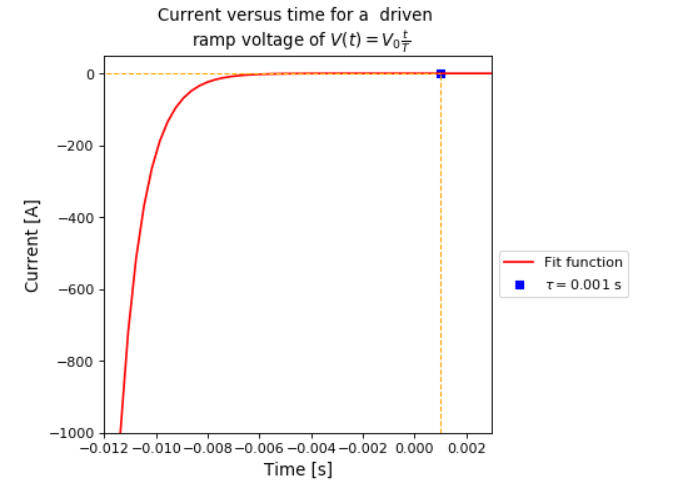
\includegraphics[width=\linewidth]{plot_phys241_ass3_1.png}
				\caption{Visual representation of the current found in part a) along with indication for the transient time.}
			\end{figure}
		\section*{Question 2.}
			\subsection*{a) }
				\begin{gather*}
					\Re{3 + j5} = 3\quad, \Im{3 + j5} = 5\\
					\abs{3+5j} = \sqrt{9+ 25} = \sqrt{34}\\
					\tan \phi = \frac{5}{3} \implies \phi = \arctan\left(\frac53\right).
				\end{gather*}
			\subsection*{b) }
				\begin{gather*}
					\Re{2j} = 0 \quad, \Im{2j} = 2\\
					\abs{2j} = \sqrt{0+4} = 2\\
					\phi = \arctan \left(\frac{2}{0^{+}}\right) = \pi/2 .
				\end{gather*}
			\subsection*{c) }
				\begin{gather*}
					\frac{1}{2-3j} = \frac{2+3j}{2-3j} = \frac{2}{13} + \frac{3}{13}j.\\
					\implies \Re{\frac{1}{2-3j}} = \frac{2}{13} \quad, \Im{\frac{1}{2-3j}} = \frac{3}{13}.\\
					\abs{\frac{1}{2-3j}} = \abs{\frac{1}{2-3j} \frac{2+3j}{2-3j}} = \abs{\frac{2+3j}{4+9}} = \frac{\abs{2+3j}}{13} = \frac{1}{\sqrt{13}}.\\
					\phi = \arctan \left(\frac32\right)
				\end{gather*}
			\subsection*{d) }
				\begin{gather*}
					3e^{j\frac{\pi}{4}} = \abs{3}(\cos(\pi/4) + j \sin(\pi/4))\\
					\implies \Re{3e^{j\frac{\pi}{4}}} = 3\cos(\pi/4) \quad , \Im{3e^{j\frac{\pi}{4}}} = 3\sin(\pi/4).\\
					\abs{3e^{j\frac{\pi}{4}}} = 3\\
					\phi = \frac{\pi}{4}.
				\end{gather*}
		\section*{Question 3.}
			\begin{gather*}
				\text{Assume } \ \widetilde{I}(t) = I_{0} e^{j(\omega t + \phi_{0})} \implies \widetilde{I}^{\p}(t) = I_{0}j\omega e^{j(\omega t + \phi_{0})}\\
				\implies LI_{0}j\omega e^{j(\omega t + \phi_{0})} = \widetilde{V}_{L} \\
				\implies Lj\omega \widetilde{I} = \widetilde{V}_{L} \implies \widetilde{I} = \frac{\widetilde{V}}{Lj\omega} \\
				\therefore Z_{C} = Lj\omega .
			\end{gather*}
		\section*{Question 4.}
			\subsection*{a) }
				The impedence for a capacitor and a resistor are respectively 
				$$ Z_{C} = \frac{1}{j\omega C} \quad, Z_{R}= R.$$
				We want the the driven sine wave to lower by one half i.e, $V^{\p} / V = 1/2.$ We have
				\begin{align*}
					\frac{V^{\p}}{V} = \frac{1}{2} = \frac{Z_{C}}{Z_{R} + Z_{C}} = \frac{\frac{1}{j\omega C}}{R + \frac{1}{j \omega C}} = \frac{1}{1+j\omega\tau}.
				\end{align*}
				\begin{gather*}
					\abs{\frac{V_{0}^{\p}}{V_{0}}} = \left(\frac{1}{1+j\omega \tau} \right)\left(\frac{1}{1-j\omega \tau}\right)= \frac{1}{1+(\omega\tau)^{2}}\\
					\implies \frac{V_{0}^{\p}}{V_{0}} = \frac{1}{\sqrt{1+ (\omega\tau)^{2}}} \\
					\therefore \frac12 = \frac{1}{\sqrt{1+ (\omega\tau)^{2}}} \implies \tau = \frac{\sqrt{3}}{\omega} = \frac{\sqrt{3}T}{2\pi}.
				\end{gather*}
			\subsection*{b) }
				It was found in part a) that 
				$$ \frac{V^{\p}}{V} = \frac{1}{1+j\omega\tau}.$$
				Let us convert this expression to extract a real and imaginary part, 
				\begin{gather*}
					\frac{1}{1+j\omega\tau} = \frac{1}{1+j\omega\tau} \left(\frac{1-j\omega\tau}{1-j\omega\tau}\right)= \frac{1-j\omega\tau}{1+(\tau\omega)^{2}} \\
					\therefore 	\frac{1}{1+j\omega\tau} = \frac{1}{1+(\omega\tau)^{2}} -j \frac{\omega\tau}{1+(\omega\tau)^{2}}.
				\end{gather*}
				By definition , 
				$$ \phi = \arctan \frac{\Im{\frac{V^{\p}}{V}}}{\Re{\frac{V^{\p}}{V}}}$$
				Substituting the previous result and whilst replacing $\phi$ by $-\pi/8$ we can solve for $\tau$ 
				\begin{gather*}
					\tan\left(\frac{-\pi}{9}\right)\left(\frac{1}{\omega}\right) = \tau.
				\end{gather*}
		\section*{Question 5.}
			\subsection*{a) }
				Let $V_{0}\cos \omega t = V_{0}e^{j\omega t}.$
				\begin{gather*}
					\widetilde{I}\widetilde{I}^{\star} = \left(\frac{V_{0}e^{j\omega t}}{R+j\omega L}\right)\left(\frac{V_{0}e^{-j\omega t}}{R-j\omega L}\right) = \frac{V_{0}^{2}}{R^{2}-j^{2}(\omega L)^{2}} = \frac{V_{0}^{2}}{R^{2} + (\omega L)^{2}}. \\
					= \frac{V_{0}^{2} / R^{2}}{1+(\omega\tau )^{2}} = \left(\frac{V_{0}^{2}}{R}\right) \frac{1}{1+(\omega\tau)^{2}} \implies \abs{\widetilde{I}} = \frac{1}{\sqrt{1+(\omega\tau)^{2}}}.
				\end{gather*}
				Let us find the offset associated with this complex current.
				\begin{gather*}
					\frac{V_{0}e^{j\omega t}}{R+j\omega L } = \frac{V_{0}}{R} \frac{e^{j\omega t}}{1+ j\omega \tau} = \frac{V_{0}}{R} \underbrace{\left(\frac{1}{1+j\omega\tau}\right)}_{= Z} e^{j\omega t}\\
					\frac{1}{1+j\omega\tau} \left(\frac{1-j\omega\tau}{1+j\omega\tau}\right) = \frac{1-j\omega\tau}{1+(\omega\tau)^{2}} = \frac{1}{1+(\omega\tau)^{2}} - j \frac{\omega\tau}{1+(\omega\tau)^{2}}\\
					\implies \phi = \arctan\left(\omega\tau\right)
				\end{gather*}
				Finally, 
				\begin{gather*}
					\widetilde{I} = \frac{V_{0}}{R} \frac{e^{j(\omega t + \phi)}}{\sqrt{1+(\tau\omega)^{2}}} \implies I(t) = \frac{V_{0}}{R} \frac{\cos(\omega t + \phi)}{\sqrt{1+(\omega\tau)^{2}}}
				\end{gather*}
			\subsection*{b) }
			\begin{gather*}
				\frac{\widetilde{V}^{\p}}{\widetilde{V}} = \frac{j\omega L}{R + j\omega L } = \frac{j\omega\tau}{1 + j\omega\tau}
				\intertext{Multiplying by the conjugate both sides we get}
					\frac{\widetilde{V}^{\p}}{\widetilde{V}} =\frac{(\omega\tau)^{2}}{1+ (\omega\tau)^{2}} \implies \widetilde{V}^{\p} = \frac{V_{0}e^{j\omega t}(\omega\tau)^{2}}{1+(\omega\tau)^{2}}.
			\end{gather*}
			Let us find the offset phase ,
			\begin{gather*}
					\frac{\widetilde{V}^{\p}}{\widetilde{V}} = \frac{j\omega \tau}{1 + j\omega\tau} = \frac{1}{1+ \frac{1}{j\omega \tau}} \\
					\implies \left(\frac{1}{1-\frac{j}{\omega\tau}}\right)\left(\frac{1+ \frac{j}{\omega\tau}}{1+\frac{j}{\omega\tau}}\right) = \frac{(\omega\tau)^{2}}{1+(\omega\tau)^{2}} + j \frac{\omega\tau}{1+(\omega\tau)^{2}} 
					\implies \phi = \frac{1}{\omega\tau}.\\
				\text{Finally, } \ \ \widetilde{V}^{\p} = \frac{V_{0}e^{j\omega t}(\omega\tau)^{2}}{1+(\omega\tau)^{2}} \\
				\therefore \frac{V_{0}\cos(\omega\tau + \frac{1}{\omega\tau})}{1+(\omega\tau)^{2}} = V^{\p}. 
			\end{gather*}
		\subsection*{c) }
			\begin{figure}[h]
						\centering
							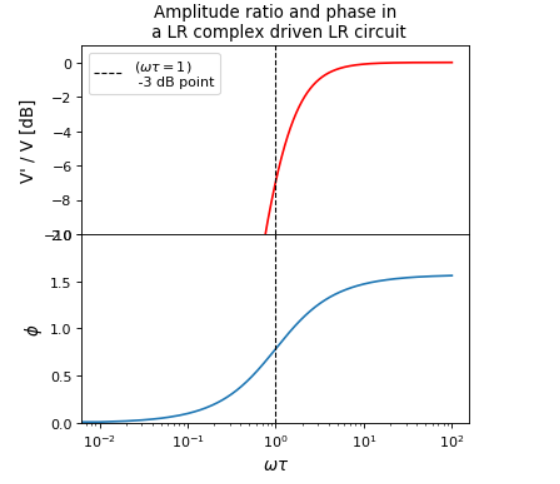
\includegraphics[width=0.8\linewidth]{plot_phys241_ass3_2.png}
							\caption{Visual representation of the ratio between the $V^{\p}$ potential and $V$, along with the evolution of $\phi$ with respect to the independent variable $\omega \tau$.}					
						\end{figure}
			
	\end{document}